\documentclass[11pt]{article}

\usepackage[margin=1in]{geometry}
\usepackage{amsmath,amssymb,amsthm}
\usepackage{booktabs}
\usepackage{enumitem}
\usepackage{graphicx}
\usepackage{hyperref}
\usepackage{placeins}
\usepackage{xcolor}

\hypersetup{
  colorlinks=true,
  linkcolor=blue,
  citecolor=blue,
  urlcolor=blue
}

\newtheorem{definition}{Definition}
\newtheorem{proposition}{Proposition}
\newtheorem{remark}{Remark}

\newcommand{\R}{\mathbb{R}}
\newcommand{\Cov}{\operatorname{Cov}}
\newcommand{\spanop}{\operatorname{span}}

\title{A Compact Narrative for Task-Visible Operator Mechanisms}
\author{Fernando Ruiz Mazo}
\date{May 1, 2026}

\begin{document}

\maketitle

\section{The Question}

The starting point is a simple ambiguity. A transformer trained for in-context linear regression may
make predictions close to linear-kernel ridge regression, but pointwise accuracy on one sampled
label vector does not identify the computation being used. Many algorithms can agree with ridge
regression on the realized labels while responding differently to nearby counterfactual labels.

The note therefore changes the object of study. Instead of asking only whether the transformer
predicts the right targets for one sampled context, it freezes the input geometry and perturbs only
the context labels. The first question becomes:
\[
\text{When labels are changed infinitesimally, does the transformer respond like the ridge operator?}
\]
This operator-response test is only the entry point. The paper then asks a stronger mechanistic
question: if the transformer has a ridge-like local response, is that response mediated by a compact
context-side activation subspace, does the subspace have the dimension predicted by the
task-visible ridge spectrum, and are the high-leverage directions in that subspace causally used?

The resulting claim is stronger than behavioral imitation but narrower than global equality. In the
tested regime, the transformer locally realizes the task-distributed ridge label-response operator;
that behavior is explained by a reduced KRR operator induced by activation-derived directions; the
number of required directions is predicted before looking at activations; and removing the
task-important directions selectively damages the response. The locality matters: the tests concern
the sampled geometry, the chosen perturbation scale, and especially the task-label directions rather
than all possible label perturbations.

\section{Fixed Geometry Makes Ridge Regression an Operator}

Fix one in-context episode with context and target inputs
\[
X_{\mathrm{ctx}}\in\R^{n_{\mathrm{ctx}}\times d_x},
\qquad
X_{\mathrm{tgt}}\in\R^{n_{\mathrm{tgt}}\times d_x}.
\]
The fixed geometry is
\[
G=(X_{\mathrm{ctx}},X_{\mathrm{tgt}}).
\]
During the operator tests, \(G\) is held fixed. The context inputs do not move, the target inputs do
not move, and the only varying object is the context-label vector
\[
y=(y_1,\ldots,y_{n_{\mathrm{ctx}}})\in\R^{n_{\mathrm{ctx}}}.
\]
Define
\[
K=X_{\mathrm{ctx}}X_{\mathrm{ctx}}^\top,\qquad
K_t=X_{\mathrm{tgt}}X_{\mathrm{ctx}}^\top,\qquad
A=K+\sigma^2 I.
\]
For linear-kernel ridge regression, the dual coefficients and target predictions are
\[
\alpha^\star=A^{-1}y,\qquad
y^\star=K_t\alpha^\star=K_tA^{-1}y.
\]
Thus, once \(G\) is fixed, ridge regression is a linear map from context labels to target
predictions:
\[
T_G:=K_tA^{-1},
\qquad
T_G:\R^{n_{\mathrm{ctx}}}\to\R^{n_{\mathrm{tgt}}}.
\]

The transformer defines a map on the same spaces:
\[
F_\theta^G:\R^{n_{\mathrm{ctx}}}\to\R^{n_{\mathrm{tgt}}},
\qquad
F_\theta^G(y)=\widehat y_\theta.
\]
When the geometry is clear, write \(T\) and \(F\). The central comparison is not merely
\(F(y)\approx Ty\) for one \(y\). It is whether the local response of \(F\) to label perturbations
matches the operator \(T\).

\section{Context-Label Directions, Local Operators, and Additivity}

A context-label direction is a vector
\[
u\in\R^{n_{\mathrm{ctx}}}.
\]
It assigns one scalar to each context example. Perturbing in direction \(u\) means changing labels as
\[
y+\varepsilon u
=
(y_1+\varepsilon u_1,\ldots,y_{n_{\mathrm{ctx}}}+\varepsilon u_{n_{\mathrm{ctx}}}).
\]
This is a direction over context positions. It is not a direction in input-feature space and not a
direction in target space. If there are 47 context examples, these directions live in \(\R^{47}\).

Pointwise agreement checks only the value of two maps at one label vector:
\[
F(y)\approx Ty.
\]
Since fixed-geometry ridge regression is linear, its Jacobian is the operator itself:
\[
J_T(y)=T\quad\text{for every }y.
\]
The transformer map \(F\) can be nonlinear in the labels. The weakest local version of ``the same
label-to-prediction rule'' is therefore equality of first-order responses:
\[
J_F(y)u\approx Tu.
\]
Equivalently, for small label perturbations,
\[
F(y+\delta)\approx F(y)+T\delta.
\]
The experiments estimate the Jacobian action with the central finite difference
\[
D_\varepsilon F(y)[u]
:=
\frac{F(y+\varepsilon u)-F(y-\varepsilon u)}{2\varepsilon}.
\]
The symmetric form is used because it cancels the leading first-order bias of a one-sided
difference: for a smooth map, the error is \(O(\varepsilon^2)\) rather than \(O(\varepsilon)\). It also
treats positive and negative label perturbations in the same direction symmetrically, which is
important when the goal is to estimate the local tangent response rather than a one-sided effect.
The behavioral operator test asks whether
\[
D_\varepsilon F(y)[u]\approx Tu
\]
on held-out label directions.

This is still a local statement. Matching the value and first derivative at one point does not imply
global equality. For example, \(f(x)=x+x^2\) and \(g(x)=x\) have the same value and derivative at
\(x=0\), but differ away from zero. Thus derivative matching supports tangent-level agreement,
not \(F(y')=Ty'\) for all possible labels.

The probe distribution specifies which counterfactual label directions are tested. The main probes
are task-label probes:
\[
u\sim\mathcal{N}(0,A).
\]
This is the natural law because, under the matched linear task
\[
y=X_{\mathrm{ctx}}\beta+\eta,\qquad
\beta\sim\mathcal{N}(0,I),\qquad
\eta\sim\mathcal{N}(0,\sigma^2I),
\]
conditioning on the fixed geometry leaves only \(\beta\) and \(\eta\) random, so
\[
y\mid G\sim\mathcal{N}(0,X_{\mathrm{ctx}}X_{\mathrm{ctx}}^\top+\sigma^2I)
=\mathcal{N}(0,A).
\]
Equivalently, the conditional label covariance is
\[
\Cov(y\mid G)=A.
\]
Thus \(u\sim\mathcal{N}(0,A)\) samples counterfactual label perturbations with the same covariance
geometry as labels generated by the task, after the input geometry has been fixed. In this precise
sense, task probes are the directions the task distribution itself emphasizes. In whitened coordinates,
they are \(u=A^{1/2}z\), \(z\sim\mathcal{N}(0,I)\). The experiments also use isotropic probes
\[
u\sim\mathcal{N}(0,I),
\]
which test arbitrary context-label directions equally. The distinction is central: the claim is
task-local because the transformer is close to ridge on task-label probes but not on arbitrary
isotropic probes. Build probes are used to construct subspaces or fitted controls; held-out probes
are used for reported errors.

For a held-out probe set \(U=\{u_1,\ldots,u_m\}\) and a fixed linear operator
\(S:\R^{n_{\mathrm{ctx}}}\to\R^{n_{\mathrm{tgt}}}\), define
\[
E_\varepsilon(F,S;U)
:=
\left(
\frac{
\sum_{j=1}^m\|D_\varepsilon F(y)[u_j]-Su_j\|_2^2
}{
\sum_{j=1}^m\|Tu_j\|_2^2+\eta_{\mathrm{num}}
}
\right)^{1/2}.
\]
When \(S=T\), this measures whether the transformer's finite-difference response matches exact
ridge regression. The denominator normalizes by the ridge-response energy on the same probes, so
an error of \(0.01\) means a root-mean-square discrepancy of about one percent of the typical ridge
response size.

\begin{proposition}[Transformer errors are not bounded by 1]
For a finite probe set \(U\), write
\[
R_U^2=\sum_j\|Tu_j\|_2^2.
\]
If \(D_\varepsilon F(y)[u_j]=0\) for all probes, then
\[
E_\varepsilon(F,T;U)=\frac{R_U}{(R_U^2+\eta_{\mathrm{num}})^{1/2}}\le 1.
\]
If \(D_\varepsilon F(y)[u_j]=-Tu_j\), then the same calculation gives a value at most 2. More
generally, if \(D_\varepsilon F(y)[u_j]=cTu_j\), then
\[
E_\varepsilon(F,T;U)
=
|c-1|\frac{R_U}{(R_U^2+\eta_{\mathrm{num}})^{1/2}},
\]
so transformer-response errors have no universal upper bound.
\end{proposition}

\begin{proof}
Substitute the three proposed finite-difference responses into the definition of
\(E_\varepsilon(F,T;U)\). The last expression diverges as \(|c|\to\infty\) whenever the ridge
response energy \(R_U^2\) is nonzero.
\end{proof}

Because ridge is linear, its higher-order derivatives are zero. We do not try to estimate all
higher-order derivatives of the transformer. Instead, we check whether nonlinear interactions are
small at the tested perturbation scale. Ridge has
\[
T(u+v)=Tu+Tv.
\]
A nonlinear transformer need not satisfy
\[
D_\varepsilon F(y)[u+v]\approx D_\varepsilon F(y)[u]+D_\varepsilon F(y)[v].
\]
If this approximate additivity failed badly, then \(E_\varepsilon(F,T)\) would mix two effects:
failure to be ridge and failure to have a stable local linear response.

For paired directions \(V=\{(u_j,v_j)\}_{j=1}^m\), define the second mixed finite difference
\[
C_j =
F(y+\varepsilon u_j+\varepsilon v_j)
-F(y+\varepsilon u_j-\varepsilon v_j)
-F(y-\varepsilon u_j+\varepsilon v_j)
+F(y-\varepsilon u_j-\varepsilon v_j),
\]
and the additivity defect
\[
A_\varepsilon(F;V)
:=
\left(
\frac{
\sum_{j=1}^m\|C_j\|_2^2
}{
\sum_{j=1}^m\|T(\varepsilon u_j+\varepsilon v_j)\|_2^2+\eta_{\mathrm{num}}
}
\right)^{1/2}.
\]
For any affine function of the labels, \(C_j=0\) exactly. Because the defect is normalized by
ridge-response energy, values below one mean the non-additive interaction is smaller than the
typical ridge response on the tested paired probes; values around one mean it is ridge-scale; values
above one mean the interaction is larger than the ridge response, so a local-linear interpretation is
unreliable. This diagnostic does not identify the operator. It only says whether a local operator
comparison is meaningful at the chosen \(\varepsilon\) and probe law.

\section{Activation Subspaces and Task-Visible Rank}

The previous section gives behavioral certificates:
\[
F(y)\approx Ty,\qquad D_\varepsilon F(y)[u]\approx Tu.
\]
These are necessary, but they are still input-output facts. They do not say whether the transformer
represents the directions needed for ridge regression, or whether those directions are used. The
mechanistic question is: does the residual stream expose a compact set of context-position
directions sufficient for the task-visible ridge computation?

This is the right internal object to look for because ridge uses context-position dual variables.
For fixed geometry,
\[
\alpha^\star(y)=A^{-1}y\in\R^{n_{\mathrm{ctx}}},
\qquad
Ty=K_t\alpha^\star(y).
\]
The dual coordinate \(\alpha_i\) is indexed by the \(i\)-th context example. The context residual
stream has the same context axis. At layer \(\ell\),
\[
H_\ell^{\mathrm{ctx}}\in\R^{n_{\mathrm{ctx}}\times D},
\]
where \(D\) is the residual width. Rows are context tokens, and the \(k\)-th column
\(H_\ell^{\mathrm{ctx}}[:,k]\) is a scalar pattern over context positions, hence a vector in
\(\R^{n_{\mathrm{ctx}}}\). Linear combinations of residual-stream columns therefore define
candidate directions in the same space as ridge dual variables.

Let
\[
Q=[q_1,\ldots,q_r]\in\R^{n_{\mathrm{ctx}}\times r}
\]
be a basis matrix for such candidate context-position directions. The subspace is the column span
\[
\spanop(Q)=\{Qc:c\in\R^r\}\subseteq\R^{n_{\mathrm{ctx}}},
\]
so \(Q\) is both a matrix representation and, by abuse of language, the subspace it spans. We use
an \(A\)-orthonormal basis,
\[
Q^\top A Q=I,
\]
because the quadratic part of the ridge dual objective is \(\frac12\alpha^\top A\alpha\). Thus the
natural size of a dual displacement is \(\alpha^\top A\alpha\), and two directions are orthogonal in
the ridge geometry when their cross-term in this quadratic energy vanishes.

Now define what it means for \(\spanop(Q)\) to be useful for ridge. This is a restriction of the
dual solution, not an ordinary restriction of the input label vector. Full ridge solves
\[
\alpha^\star(y)
=
\arg\min_{\alpha\in\R^{n_{\mathrm{ctx}}}}
\left\{
\frac12\alpha^\top A\alpha-\alpha^\top y
\right\},
\]
whose first-order condition is \(A\alpha-y=0\), hence \(\alpha^\star=A^{-1}y\). To restrict the
dual solution to \(\spanop(Q)\), write \(\alpha=Qc\). Plugging this into the same dual objective gives
\[
\frac12 c^\top Q^\top A Qc-c^\top Q^\top y.
\]
Since \(Q^\top A Q=I\), this is
\[
\frac12 c^\top c-c^\top Q^\top y.
\]
Differentiating with respect to \(c\) gives \(c-Q^\top y=0\), so
\[
c^\star=Q^\top y.
\]
Therefore the restricted dual solution is
\[
\alpha_Q(y)=QQ^\top y.
\]
Without the \(A\)-orthonormal convention, the same calculation would give
\[
\alpha_Q(y)=Q(Q^\top A Q)^{-1}Q^\top y.
\]
Predictions are still read out through the context-target kernel matrix \(K_t\), so the reduced
ridge operator induced by \(Q\) is
\[
T_Q:=K_tQQ^\top.
\]
This is the bridge from residual-stream directions to an operator-level certificate. We are not
fitting an arbitrary probe. We are asking whether the directions exposed by the residual stream are
enough so that ridge, restricted to those directions, still predicts like full ridge.

For two linear operators, define
\[
E(S_1,S_2;U)
:=
\left(
\frac{
\sum_{j=1}^m\|(S_1-S_2)u_j\|_2^2
}{
\sum_{j=1}^m\|Tu_j\|_2^2+\eta_{\mathrm{num}}
}
\right)^{1/2}.
\]
Thus \(E(T_Q,T;U)\) is the reduced-operator error: it measures how much prediction response is lost
when full ridge is restricted to \(\spanop(Q)\) on the tested label directions. A small value says
that \(Q\) is sufficient for ridge in this operator sense. It does not yet say that the transformer
uses \(Q\).

The reason this sufficiency test is task-visible rather than global is that not every label direction
matters equally for prediction. Conditional on the fixed geometry,
\[
y\mid G\sim\mathcal{N}(0,A).
\]
So the task naturally emphasizes perturbations
\[
u\sim\mathcal{N}(0,A),
\]
not arbitrary Euclidean directions. A direction is task-relevant when it is likely under this
covariance geometry and when ridge produces a non-negligible target response along it. This leads
to a purely ridge-theoretic benchmark: before looking inside the transformer, ask how many
directions are needed by the best possible reduced ridge response on task-distributed labels.

For a rank-\(r\) linear operator \(S_r:\R^{n_{\mathrm{ctx}}}\to\R^{n_{\mathrm{tgt}}}\), define
\[
\mathcal{E}_r(G)^2
:=
\inf_{\operatorname{rank}(S_r)\le r}
\frac{
\mathbb{E}_{u\sim\mathcal{N}(0,A)}\|Tu-S_ru\|_2^2
}{
\mathbb{E}_{u\sim\mathcal{N}(0,A)}\|Tu\|_2^2+\eta_{\mathrm{num}}
}.
\]
This asks: if only \(r\) independent label directions can affect the target prediction, what is the
smallest relative mean squared prediction error one could achieve on task-label perturbations?

To compute this number, whiten the task-label perturbations:
\[
u=A^{1/2}z,\qquad z\sim\mathcal{N}(0,I).
\]
Then
\[
Tu=K_tA^{-1}A^{1/2}z=K_tA^{-1/2}z.
\]
Define
\[
C_G:=K_tA^{-1/2}.
\]
This is the ridge response in coordinates where task-label perturbations are isotropic. Singular
values of \(T\) would answer the wrong question: they measure response size for raw isotropic
directions \(u\sim\mathcal{N}(0,I)\). Singular values of \(C_G\) measure response size for the task
law \(u\sim\mathcal{N}(0,A)\).

Let
\[
C_G=U\operatorname{diag}(s_i)V^\top,
\qquad
s_1\ge s_2\ge\cdots\ge0.
\]
In whitened direction \(v_i\), the ridge prediction changes by \(s_i u_i\), so \(s_i^2\) is the
squared prediction-change size associated with that task direction. Since \(z\) is isotropic,
\[
\mathbb{E}\|C_Gz\|_2^2=\sum_i s_i^2.
\]
The best rank-\(r\) approximation keeps the \(r\) largest singular directions, and the omitted
prediction error is the tail:
\[
\mathcal{E}_r(G)^2
=
\frac{\sum_{i>r}s_i^2}{\sum_i s_i^2+\eta_{\mathrm{num}}}.
\]
Equivalently, the numerator is the smallest possible average squared prediction error after keeping
only \(r\) task-visible directions, and the denominator is the average squared ridge prediction
change.

\begin{definition}[Task-visible rank]
For fixed geometry \(G\) and tolerance \(\epsilon>0\), define
\[
r_{\mathrm{task}}(G;\epsilon)
:=
\min\left\{
r:
\frac{\sum_{i>r}s_i^2}{\sum_i s_i^2+\eta_{\mathrm{num}}}
\le \epsilon^2
\right\}.
\]
\end{definition}

Thus \(r_{\mathrm{task}}\) is not the algebraic rank of \(T\). It is the number of ridge-relevant
directions needed so that the best reduced response has relative mean squared prediction error at
most \(\epsilon^2\) on the task-label distribution. If \(\dim\spanop(Q)<r_{\mathrm{task}}\), then no
rank-\(\dim\spanop(Q)\) operator, even an optimally aligned one, can reach that tolerance on task
probes. If \(\dim\spanop(Q)\ge r_{\mathrm{task}}\), success is still not automatic: the span must also
align with the task-visible ridge directions.

For the linear kernel,
\[
\operatorname{rank}(C_G)
=\operatorname{rank}(T)
=\operatorname{rank}(K_t)
\le \min\{d_x,n_{\mathrm{ctx}},n_{\mathrm{tgt}}\},
\]
because \(A\) is invertible and \(K_t=X_{\mathrm{tgt}}X_{\mathrm{ctx}}^\top\). Hence
\[
r_{\mathrm{task}}(G;\epsilon)
\le \min\{d_x,n_{\mathrm{ctx}},n_{\mathrm{tgt}}\}.
\]
In the flat random linear geometries used in the target-rank sweep, this upper bound is typically
attained at the reported tolerance. Writing \(X_{\mathrm{ctx}}=P\Sigma V^\top\),
\[
C_G
=X_{\mathrm{tgt}}V\,
\operatorname{diag}\!\left(\frac{\sigma_i}{\sqrt{\sigma_i^2+\sigma^2}}\right)P^\top .
\]
With \(n_{\mathrm{ctx}}=47\) and \(\sigma^2=0.1\), the context singular values are typically much
larger than the ridge noise, so the shrinkage factors are close to one. When
\(d_x\le n_{\mathrm{tgt}}=16\), the target-side factor \(X_{\mathrm{tgt}}V\) is generically full column
rank, so the task-visible rank is empirically close to \(d_x\). In the \(d_x=30\) stress case,
\(n_{\mathrm{tgt}}=16\) caps the task-visible rank.

\section{Nonlinear Kernels and the Sample-Size Elbow}

The task-visible rank definition does not rely on the linear kernel. For a general kernel, replace
\[
K=X_{\mathrm{ctx}}X_{\mathrm{ctx}}^\top,
\qquad
K_t=X_{\mathrm{tgt}}X_{\mathrm{ctx}}^\top
\]
by \(K_{ij}=k(x_i,x_j)\) and \((K_t)_{aj}=k(x_a^{\mathrm{tgt}},x_j)\), keep
\(A=K+\sigma^2 I\), and again form
\[
C_G=K_tA^{-1/2}.
\]
The singular spectrum of \(C_G\) is the finite-episode ridge response spectrum on task-distributed
label perturbations. Its tail defines the task-visible rank; write this rank as
\(r_T(G;\epsilon)=r_{\mathrm{task}}(G;\epsilon)\). It is the number of directions a mechanism must
represent, and align with, to implement KRR at tolerance \(\epsilon\) on that episode.

For nonlinear kernels, \(r_T\) should not be read as an input-dimension count. The finite matrix
still obeys
\[
\operatorname{rank}(C_G)\le \min\{n_{\mathrm{ctx}},n_{\mathrm{tgt}}\},
\]
but the population source of the rank is the Mercer spectrum of the kernel under the input law
\(\rho\):
\[
k(x,x')=\sum_{j\ge0}\mu_j\phi_j(x)\phi_j(x'),
\qquad
\mu_0\ge\mu_1\ge\cdots\ge0.
\]
With \(n=n_{\mathrm{ctx}}\), ridge resolves mode \(j\) with visible energy approximately
\[
e_j(n)
\asymp
\mu_j\,\frac{n\mu_j}{n\mu_j+\sigma^2}
=
\frac{\mu_j^2}{\mu_j+\sigma^2/n}.
\]
The multiplier \(n\mu_j/(n\mu_j+\sigma^2)\) is a statistical visibility factor. Modes satisfying
\[
n\mu_j\ll\sigma^2
\]
are below the ridge noise floor and contribute only weakly to the label-response operator. Modes
satisfying \(n\mu_j\gtrsim\sigma^2\) are visible. Thus the population analogue of the task-visible
rank is
\[
r_*(n;\epsilon)
:=
\min\left\{
r:
\frac{\sum_{j>r}e_j(n)}{\sum_j e_j(n)}
\le \epsilon^2
\right\}.
\]

This gives the right reading of finite ranks:
\[
r_T(G;\epsilon)
\approx
\min\{n_{\mathrm{ctx}},\,n_{\mathrm{tgt}},\,r_*(n_{\mathrm{ctx}};\epsilon)\},
\]
up to finite-sample fluctuations. The first two terms are sequence-design caps. They are not
intrinsic limitations of the kernel; they can be raised by using more context or target points. The
third term is intrinsic to the chosen kernel, input distribution, noise level, context size, and
tolerance. It is the rank of the population-visible KRR operator.

This is the sample-size elbow. Increasing \(n_{\mathrm{ctx}}\) lowers the visibility threshold
\(\sigma^2/n_{\mathrm{ctx}}\) and can reveal additional Mercer modes. Increasing
\(n_{\mathrm{tgt}}\) does not reveal new population modes, but it prevents the finite diagnostic from
being target-capped. To train or certify a transformer as implementing the full visible KRR operator
in a regime, one should choose sequence lengths so that
\[
\min\{n_{\mathrm{ctx}},\,n_{\mathrm{tgt}},\,r_*(n_{\mathrm{ctx}};\epsilon)\}
=
r_*(n_{\mathrm{ctx}};\epsilon).
\]
Otherwise the model may succeed on, and the diagnostics may certify only, a capped low-rank slice
of KRR rather than the full task-visible operator. Since \(r_*(n;\epsilon)\) depends only on the
kernel spectrum, input law, noise level, context size, and tolerance, it can be estimated before
training and used to choose the context and target lengths.

\begin{proposition}[Task-probe scale for \(T_Q\)]
Let \(u=A^{1/2}z\), \(z\sim\mathcal{N}(0,I)\), and let \(Q^\top A Q=I\). With
\[
C=K_tA^{-1/2},\qquad W=A^{1/2}Q,\qquad P_Q=WW^\top,
\]
the population task-probe error satisfies
\[
E_{\mathrm{task}}(T_Q,T)^2
=
\frac{\|C(I-P_Q)\|_F^2}{\|C\|_F^2+\eta_{\mathrm{num}}}.
\]
Hence
\[
0\le E_{\mathrm{task}}(T_Q,T)\le 1.
\]
If \(W\) spans the top \(r\) right singular directions of \(C\), then
\[
E_{\mathrm{task}}(T_Q,T)^2
=
\frac{\sum_{i>r}s_i^2}{\sum_i s_i^2+\eta_{\mathrm{num}}}.
\]
\end{proposition}

\begin{proof}
Since \(W=A^{1/2}Q\), \(W^\top W=Q^\top A Q=I\). For \(u=A^{1/2}z\),
\[
Tu=K_tA^{-1}A^{1/2}z=Cz,
\qquad
T_Qu=K_tQQ^\top A^{1/2}z=K_tA^{-1/2}WW^\top z=CP_Qz.
\]
Taking expectation over \(z\) gives
\[
\mathbb{E}\|(T-T_Q)u\|_2^2=\|C(I-P_Q)\|_F^2,
\qquad
\mathbb{E}\|Tu\|_2^2=\|C\|_F^2.
\]
Right multiplication by the projection \(I-P_Q\) cannot increase Frobenius norm, so the error is at
most 1. The singular-value expression follows from Eckart--Young: among all rank-\(r\) right
projections, the top right singular subspace of \(C\) minimizes the Frobenius residual, leaving
\(\sum_{i>r}s_i^2\).
\end{proof}

\begin{proposition}[Triangle reading]
For any fixed operator \(S\),
\[
E_\varepsilon(F,T;U)
\le
E_\varepsilon(F,S;U)+E(S,T;U).
\]
Taking \(S=T_Q\) is the decomposition used in the experiments.
\end{proposition}

\begin{proof}
Stack the probe responses as columns. The three numerators are Frobenius norms of
\(M_F-M_T\), \(M_F-M_S\), and \(M_S-M_T\), and all have the same denominator
\((\sum_j\|Tu_j\|_2^2+\eta_{\mathrm{num}})^{1/2}\). The result is the Frobenius triangle inequality.
\end{proof}

\begin{remark}[Reading the numbers]
For population task-probe reduced operators, \(E(T_Q,T)\in[0,1]\). An error \(e\) is a relative RMS
operator error, while \(e^2\) is the missed fraction of task-probe ridge-response energy. Thus
\(0.01\) is about one percent RMS error, \(0.1\) misses about one percent of squared response
energy, and \(0.54\) misses about \(29\%\). Values near 1 mean the reduced operator leaves almost
all task-visible ridge response unexplained. Transformer errors \(E_\varepsilon(F,T)\) and
\(E_\varepsilon(F,T_Q)\) are not bounded by 1, as noted above.
\end{remark}

The mechanism argument therefore needs three distinct checks:
\[
E_\varepsilon(F,T;U)\ \text{small},
\qquad
E(T_Q,T;U)\ \text{small},
\qquad
E_\varepsilon(F,T_Q;U)\ \text{small}.
\]
The first is behavioral. The second says the residual-stream subspace supports ridge in the
reduced-operator sense. The third says the transformer's local response follows the reduced
operator induced by that same subspace. The decomposition
\[
D_\varepsilon F(y)[u]-Tu
=
\bigl(D_\varepsilon F(y)[u]-T_Qu\bigr)
+
\bigl(T_Qu-Tu\bigr)
\]
keeps these claims separate.

It remains to describe how the residual-stream subspace is extracted. The experiments use two
final-state constructions in this section, and the next section introduces the causal layerwise
construction. Given any context-pattern
matrix \(M\in\R^{n_{\mathrm{ctx}}\times p}\), compute the \(A\)-weighted SVD
\[
A^{1/2}M=U\Sigma V^\top,
\]
keep the selected left singular directions, and map back:
\[
Q(M):=A^{-1/2}U_{\mathrm{kept}}.
\]
Then \(Q(M)^\top A Q(M)=I\). The kept singular directions are those above the numerical threshold
or within the predeclared rank budget. The task-visible rank tells how many ridge-relevant
directions should be enough in principle; the experiments then ask whether the residual-stream
directions achieve small \(E(T_Q,T)\) around that scale.

The raw final-state extractor uses the unperturbed final residual stream,
\[
M_{\mathrm{raw}}=H_L^{\mathrm{ctx}},
\qquad
Q_{\mathrm{raw}}:=Q(M_{\mathrm{raw}}).
\]
It asks an availability question: which context-position directions are linearly visible in the final
residual stream, and are enough of them present to support the task-visible ridge operator?

The response-only extractor uses finite-difference changes in the final residual stream,
\[
Z_L(u)=
\frac{
H_L^{\mathrm{ctx}}(y+\varepsilon u)-H_L^{\mathrm{ctx}}(y-\varepsilon u)
}{2\varepsilon},
\qquad
M_{\mathrm{resp}}=[Z_L(u_1),\ldots,Z_L(u_m)],
\]
and sets
\[
Q_{\mathrm{resp}}:=Q(M_{\mathrm{resp}}).
\]
It asks the stricter question: among the directions that actually move when labels are perturbed,
is there a context-position subspace whose induced \(T_Q\) is close to ridge?

In both constructions \(Q\) is frozen after extraction. If the basis were re-extracted for each
held-out perturbation, it would not define one stable reduced operator. The certificate is that a
fixed subspace extracted from residual-stream activations induces a fixed \(T_Q\) that agrees with
ridge and with the transformer's held-out local response.

\section{Causal Layerwise Construction}

The final-state certificate can show that a useful subspace is present at the end of the computation,
but it does not explain how that subspace appears across layers. The layerwise construction is a
post-training diagnostic for this question. It looks for context-side directions that satisfy three
conditions: they move when labels are perturbed, they are new relative to what earlier layers have
already supplied, and they are causally useful for the transformer's response.

The reported dimension counts only directions that are directly accepted from residual-stream
responses.

At layer \(\ell\), define the hidden-state finite-difference response
\[
Z_\ell(u)
:=
\frac{
H_\ell^{\mathrm{ctx}}(y+\varepsilon u)-H_\ell^{\mathrm{ctx}}(y-\varepsilon u)
}{2\varepsilon}.
\]
Stacking these matrices over build probes gives
\[
M_\ell=[Z_\ell(u_1),\ldots,Z_\ell(u_m)].
\]
The columns of \(M_\ell\) are context-position patterns that are visible at layer \(\ell\) when
context labels move. This is the first filter: a direction that does not appear in label-induced
hidden-state changes is not counted as part of the label-computation mechanism.

The second filter prevents double-counting. Define the accepted direction matrices inductively.
Initialize with no accepted directions. At the beginning of layer \(\ell\), assume that
\[
S_0,\ldots,S_{\ell-1}
\]
have already been defined, where \(S_j\) is the matrix of directions first accepted at layer \(j\)
and is empty if none were accepted. Declare as already available the seed span generated by these
earlier accepted directions:
\[
R_\ell^{\mathrm{pre}}
:=
\spanop\{S_j:0\le j<\ell\},
\]
where the span is over the columns of these matrices. For \(\ell=0\), this span is empty. Projection
and orthogonality are measured in the \(A\)-geometry, because the candidate directions are later used
to define the reduced ridge operator.

Let \(Q_\ell^{\mathrm{pre}}\) be an \(A\)-orthonormal basis for this pre-existing span. The novel
component of the layer response is
\[
N_\ell
=
\left(I-Q_\ell^{\mathrm{pre}}(Q_\ell^{\mathrm{pre}})^\top A\right)M_\ell.
\]
Thus \(N_\ell\) is the label-sensitive layer response after removing directions already accepted
from earlier layers. Later layers do not receive credit for re-exposing the same context-position
direction.

An \(A\)-weighted SVD of \(N_\ell\) proposes candidate directions
\[
A^{1/2}N_\ell=U_\ell\Sigma_\ell V_\ell^\top,
\qquad
q_i=A^{-1/2}U_{\ell,i}.
\]
These candidates are visible and novel, but visibility is still not use.

The third filter is causal. For each candidate \(q_i\), remove its \(A\)-orthogonal projection from
the context residual stream at layer \(\ell\):
\[
H_\ell^{\mathrm{ctx}}
\longmapsto
H_\ell^{\mathrm{ctx}}-q_iq_i^\top A H_\ell^{\mathrm{ctx}},
\]
roll the remaining layers forward, and measure the damage to the finite-difference response on a
separate causal-probe set. A candidate is accepted only if this damage exceeds a predeclared
threshold. Let \(I_\ell\) be the accepted candidate indices. This completes the induction step by
defining
\[
S_\ell:=A^{-1/2}U_{\ell,I_\ell}.
\]
If \(I_\ell\) is empty, then \(S_\ell\) is empty. Otherwise its columns are \(A\)-orthonormal and are
the directions first accepted at layer \(\ell\). The selection rule is deliberately stronger than
decodability: a direction must be visible, novel, and functionally consequential at the tested layer.

After processing all layers, the accepted directions define the seed layerwise activation span
\[
R_{\mathrm{seed}}
:=
\spanop\{S_\ell:0\le \ell\le L\},
\qquad
d_{\mathrm{seed}}:=\dim R_{\mathrm{seed}}.
\]
Let \(Q_{\mathrm{seed}}\) be an \(A\)-orthonormal basis of this span. The induced reduced operator is
\[
T_{Q_{\mathrm{seed}}}=K_tQ_{\mathrm{seed}}Q_{\mathrm{seed}}^\top.
\]
The layerwise test then compares \(d_{\mathrm{seed}}\) to the task-visible rank and compares
\(T_{Q_{\mathrm{seed}}}\) to \(T\). The dimension \(d_{\mathrm{seed}}\) is an accounting statistic, not
the certificate by itself. It says how many directly accepted context-position directions the
checkpoint exposes. The operator error \(E(T_{Q_{\mathrm{seed}}},T)\) says whether those directions are
aligned with the task-visible ridge directions. A span may have enough dimension and still miss part
of \(T\), and a full-dimensional span can make \(T_Q=T\) trivially without implying that the
transformer behaves like ridge.

\section{Experiment 1: Final-State Operator Certificate}

Experiment 1 is the endpoint certificate. It asks two questions. First, does the trained
transformer locally behave like exact KRR at the final prediction output? Second, if it does, is
there a compact final-state context-position subspace whose induced reduced ridge operator explains
that behavior?

For each episode, the geometry \(G\) is fixed and the exact ridge operator
\[
T=K_tA^{-1}
\]
is computed. The experiment draws separate build probes and held-out evaluation probes. Build
probes are used only to extract bases or fit controls; all reported operator errors are evaluated
after the basis is frozen. In the reported run there are 4 episodes, 16 build probes, 32 held-out
evaluation probes, finite-difference scale \(\varepsilon=10^{-3}\), and a predeclared extraction rank
cap \(r_{\max}=9\).

The experiment constructs two final-state bases. The raw basis uses the unperturbed final context
residual stream
\[
M_{\mathrm{raw}}:=H_L^{\mathrm{ctx}}\in\R^{n_{\mathrm{ctx}}\times D}.
\]
Each residual coordinate is a context-position pattern, and the \(A\)-weighted SVD of
\(M_{\mathrm{raw}}\) gives an \(A\)-orthonormal basis \(Q_{\mathrm{raw}}\).

The response-only basis uses only the part of the final residual stream that moves under label
perturbations. For task-label build probes \(u_1,\ldots,u_m\), define
\[
Z_L(u_j)=
\frac{
H_L^{\mathrm{ctx}}(y+\varepsilon u_j)-H_L^{\mathrm{ctx}}(y-\varepsilon u_j)
}{2\varepsilon},
\qquad
M_{\mathrm{resp}}=[Z_L(u_1),\ldots,Z_L(u_m)].
\]
An \(A\)-weighted SVD of \(M_{\mathrm{resp}}\) gives \(Q_{\mathrm{resp}}\). This is a stricter
availability test than the raw basis: the directions must be visible in label-induced hidden-state
changes, not merely present in the final residual stream.

For either frozen basis \(Q\), the KRR-structured reduced operator is
\[
T_Q=K_tQQ^\top.
\]
The experiment evaluates both subspace sufficiency,
\[
E(T_Q,T),
\]
and model-subspace alignment,
\[
E_\varepsilon(F,T_Q).
\]

It also includes a same-span least-squares readout control, denoted \(T_{\mathrm{actLR}}\). For any
perturbation \(u\), both \(T_Q\) and this control first form the same activation coordinates
\[
z=Q^\top u.
\]
The KRR-structured reduced operator then uses the KRR-implied readout from those coordinates:
\[
T_Qu=(K_tQ)(Q^\top u),
\qquad
C_{\mathrm{KRR}}=K_tQ.
\]
The control keeps the same features \(Q^\top u\), but fits the readout directly to the
transformer's finite-difference responses on build probes \(u_1,\ldots,u_B\):
\[
C_Q\in
\arg\min_{C\in\R^{n_{\mathrm{tgt}}\times r}}
\sum_{j=1}^B
\left\|D_\varepsilon F(y)[u_j]-CQ^\top u_j\right\|_2^2.
\]
It then defines
\[
T_{\mathrm{actLR}}u=C_Q(Q^\top u),
\qquad
T_{\mathrm{actLR}}:=C_QQ^\top.
\]
Thus the two operators use the same \(Q\)-features but different readouts: \(T_Q\) uses the fixed KRR
readout \(K_tQ\), while \(T_{\mathrm{actLR}}\) uses the least-squares readout \(C_Q\) fitted to the
transformer. This control is important because it separates two questions. A good
\(T_{\mathrm{actLR}}\) fit would show that the transformer's local response is decodable from the
activation coordinates. A good \(T_Q\) fit shows something stronger: the same coordinates support
the KRR-constrained readout.

The behavioral check succeeds on task-label probes. The pointwise prediction is already close to
KRR, with relative model--KRR discrepancy \(0.01045\), and the held-out finite-difference operator
error is
\[
E_\varepsilon(F,T)=0.0121.
\]
The additivity defect is much smaller than this error: \(4.43\times10^{-4}\) on task probes and
\(3.49\times10^{-3}\) on isotropic probes at \(\varepsilon=10^{-3}\), with comparable values at
\(10\varepsilon\). Thus the local response is sufficiently close to additive for the operator
comparison to be meaningful.

The final-state subspace certificates also succeed on task probes. For the raw basis,
\[
E(T_Q,T)=0.00148,
\qquad
E_\varepsilon(F,T_Q)=0.01194.
\]
For the response-only basis,
\[
E(T_Q,T)=0.00367,
\qquad
E_\varepsilon(F,T_Q)=0.01239.
\]
So the final residual stream exposes compact context-position subspaces whose induced reduced
ridge operators are close to exact KRR, and the transformer's local response follows those reduced
operators.

The \(T_{\mathrm{actLR}}\) control shows what this certificate is not saying. On task probes,
\(T_{\mathrm{actLR}}\) fits the transformer slightly better than \(T_Q\): for the raw basis
\[
E_\varepsilon(F,T_{\mathrm{actLR}})=0.00726
\quad\text{versus}\quad
E_\varepsilon(F,T_Q)=0.01194.
\]
But it agrees worse with exact KRR:
\[
E(T_{\mathrm{actLR}},T)=0.01202
\quad\text{versus}\quad
E(T_Q,T)=0.00148.
\]
The response-only basis shows the same pattern. Therefore the certificate is not merely that a
free low-rank readout can fit the model response; it is that the same activation-derived subspace
supports the KRR-structured operator. Matched random subspaces of the same rank fail the
operator-sufficiency test by large factors on task probes, with \(E(T_Q,T)\approx0.117\) for the raw
rank and \(0.0955\) for the response rank.

The limitation appears immediately off distribution. On isotropic probes,
\[
E_\varepsilon(F,T)\approx0.302.
\]
The raw reduced operator remains closer to exact KRR than the transformer response does,
\[
E(T_Q,T)=0.0525,
\qquad
E_\varepsilon(F,T_Q)=0.2915,
\]
but the model is no longer KRR-like on arbitrary label directions. Experiment 1 therefore supports
a task-local final-state operator certificate, not a global implementation of ridge regression on
all context-label directions.

\begin{table}[htbp]
\centering
\caption{Experiment 1 predictive and behavioral checks, mean over 4 episodes.}
\begin{tabular}{lccc}
\toprule
Quantity & Transformer & Exact KRR & Transformer--KRR\\
\midrule
Pointwise MSE to noiseless teacher targets & 0.0161 & 0.0148 & --\\
Pointwise relative discrepancy & -- & -- & 0.01045\\
Held-out task operator error \(E_\varepsilon(F,T)\) & -- & -- & 0.0121\\
\bottomrule
\end{tabular}
\end{table}

\begin{table}[htbp]
\centering
\caption{Experiment 1 additivity defect, mean over 4 episodes. The defect measures the normalized
failure of finite-difference responses to add:
\(\bigl(\sum_j\|D_\varepsilon F[u_j+v_j]-D_\varepsilon F[u_j]-D_\varepsilon F[v_j]\|^2/
(\sum_j\|T(u_j+v_j)\|^2+\eta_{\mathrm{num}})\bigr)^{1/2}\).}
\begin{tabular}{lcc}
\toprule
Probe distribution & \(\varepsilon=10^{-3}\) & \(\varepsilon=10^{-2}\)\\
\midrule
Task-label probes & \(4.43\times10^{-4}\) & \(3.52\times10^{-4}\)\\
Isotropic probes & \(3.49\times10^{-3}\) & \(2.93\times10^{-3}\)\\
\bottomrule
\end{tabular}
\end{table}

\begin{table}[htbp]
\centering
\caption{Reduced operator vs. same-span response-fitted low-rank control, mean over 4 episodes.
\(E_\varepsilon(F,S)\) denotes transformer-to-\(S\) finite-difference operator error; \(E(S,T)\)
denotes \(S\)-to-ridge operator error.}
\begin{tabular}{llcccc}
\toprule
Probe distribution & Basis & \(E(F,T_Q)\) & \(E(F,T_{\mathrm{actLR}})\) & \(E(T_Q,T)\) & \(E(T_{\mathrm{actLR}},T)\)\\
\midrule
Task probes & raw & 0.01194 & 0.00726 & 0.00148 & 0.01202\\
Task probes & response & 0.01239 & 0.01169 & 0.00367 & 0.01645\\
Isotropic probes & raw & 0.2915 & 0.2007 & 0.05254 & 0.2687\\
Isotropic probes & response & 0.3193 & 0.2418 & 0.1278 & 0.2929\\
\bottomrule
\end{tabular}
\end{table}

The three plots below should be read as diagnostic decompositions of the same certificate.  In all
of them the vertical axis is a relative error on a logarithmic scale, so lower is better and equal
vertical gaps correspond to multiplicative changes.  The word ``label'' in the plot labels means
task-label probes, \(u\sim N(0,A)\); ``isotropic'' means \(u\sim N(0,I)\).  The first plot asks
whether a free response fit from the same coordinates gives the same conclusion as the
KRR-constrained reduced operator.  The second plot asks how the certificate changes as we move
continuously from task-label probes to isotropic probes.  The third plot asks how much retained
rank is needed before the final-state basis supports the task-visible ridge computation.

\begin{figure}[htbp]
\centering
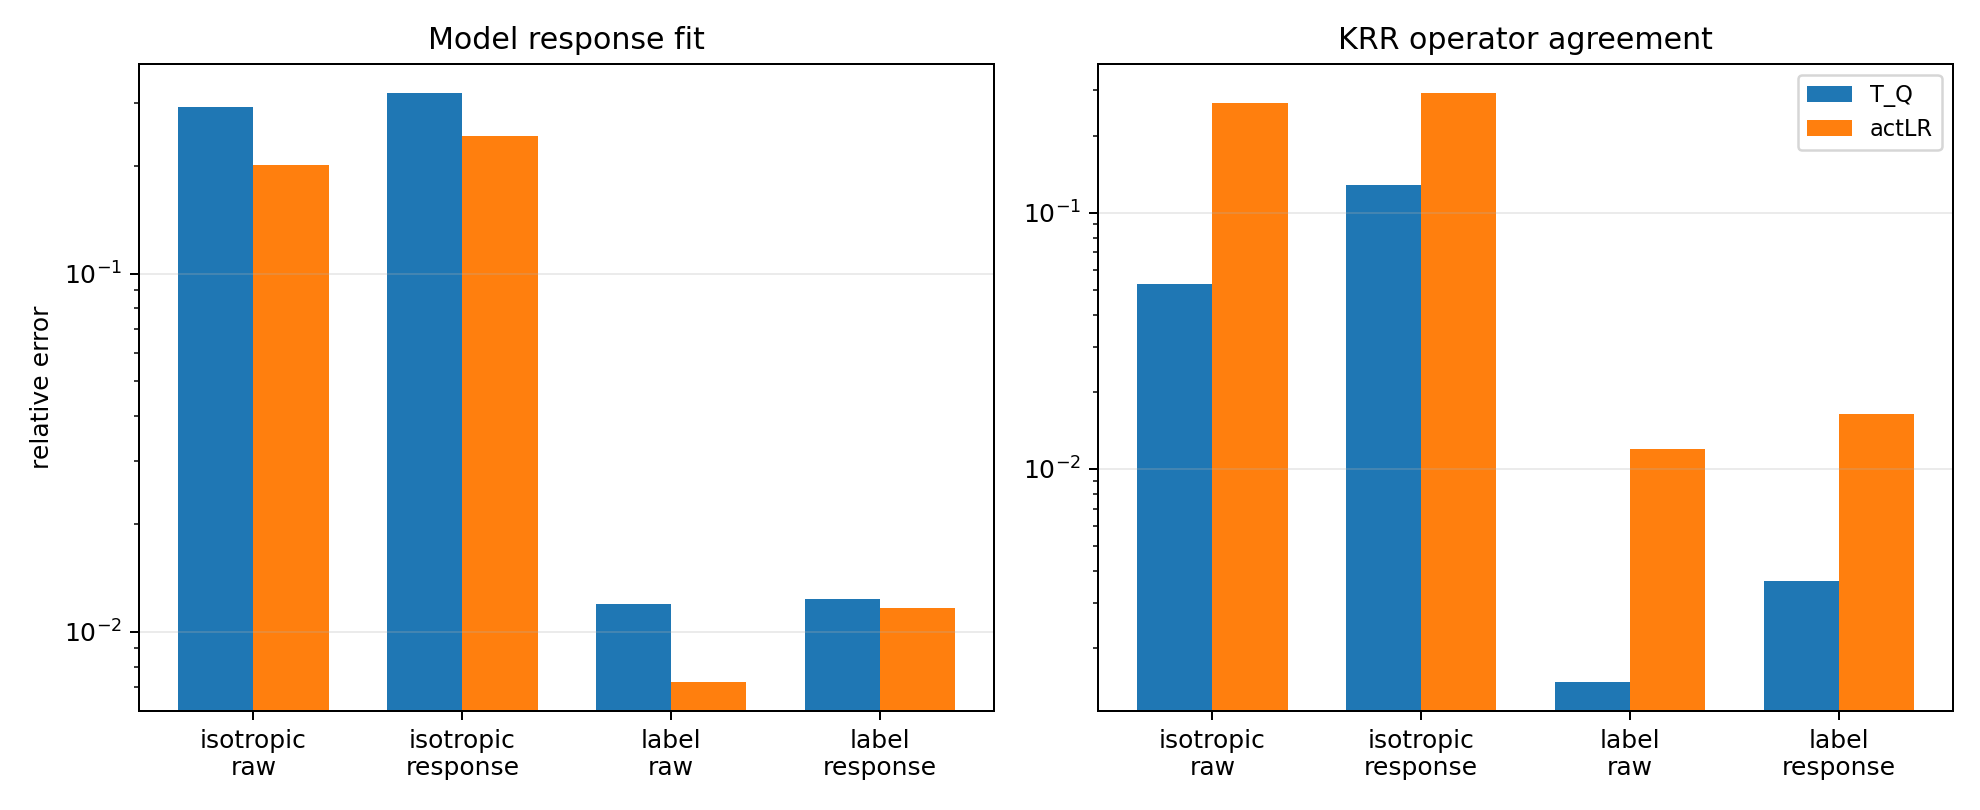
\includegraphics[width=\linewidth]{../experiments/exp1_operator_certificate/results/actlr_comparison.png}
\caption{Experiment 1 reduced-operator certificate versus same-span response fitting. Left panel:
transformer-to-operator response error \(E_\varepsilon(F,S)\), where \(S=T_Q\) for the
KRR-constrained reduced operator and \(S=T_{\mathrm{actLR}}\) for the same-span response-fitted
control.  This panel measures only how well the candidate operator predicts the transformer's
finite-difference responses.  Right panel: operator-to-ridge error \(E(S,T)\), which measures
whether the candidate operator is actually close to exact KRR.  Thus a good mechanistic
certificate should be low in both panels.  The free response-fitted operator improves the left
panel on task probes, especially for the raw basis, but it is worse in the right panel; it fits the
model slightly better by giving up KRR structure.  The KRR-constrained \(T_Q\) is therefore the
stronger ridge certificate.}
\end{figure}

\begin{figure}[htbp]
\centering
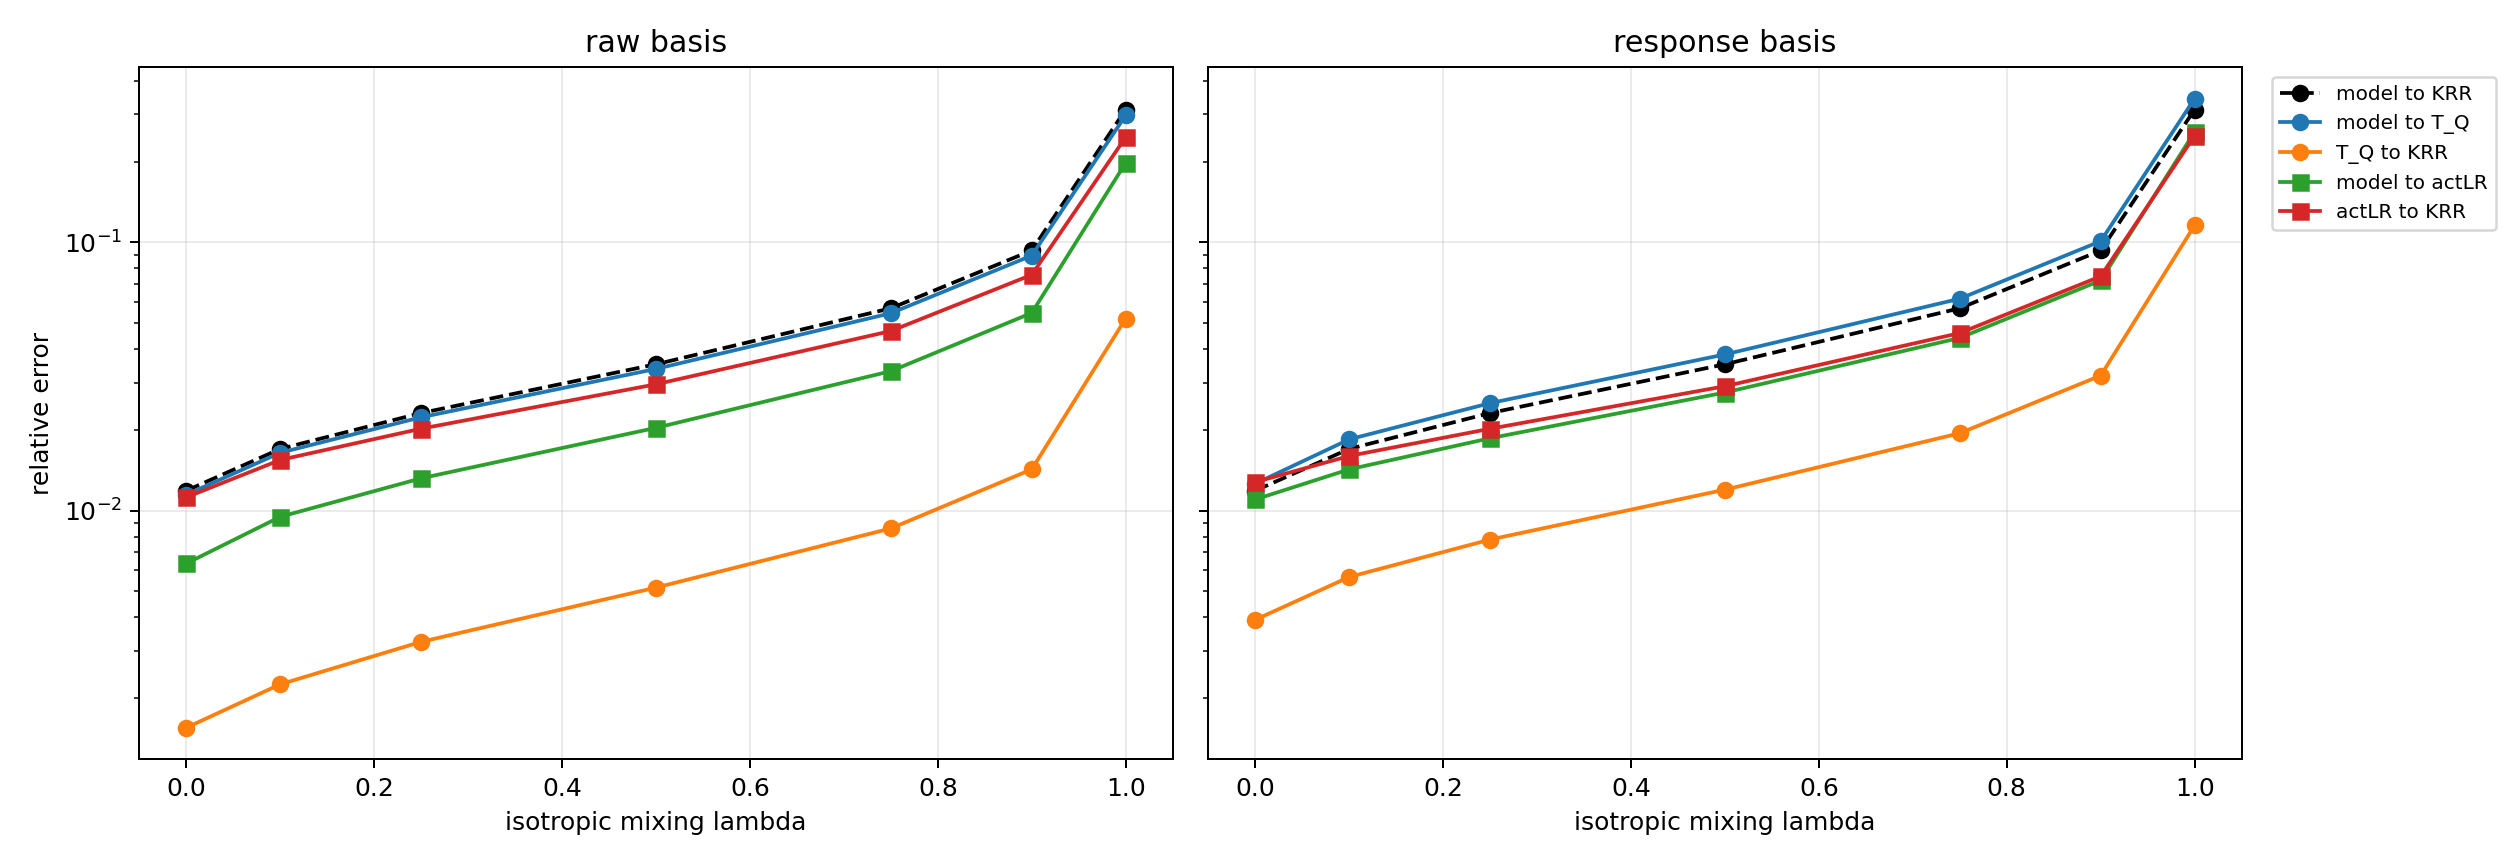
\includegraphics[width=\linewidth]{../experiments/exp1_operator_certificate/results/probe_interpolation.png}
\caption{Experiment 1 probe interpolation. The horizontal axis is the probe mixing parameter
\(\lambda\), where probes are drawn as
\(u_\lambda=\sqrt{1-\lambda}\,u_{\mathrm{task}}+\sqrt{\lambda}\,u_{\mathrm{iso}}\), with
\(u_{\mathrm{task}}\sim N(0,A)\) and \(u_{\mathrm{iso}}\sim N(0,I)\).
Thus \(\lambda=0\) is the task-label regime and \(\lambda=1\) is the fully isotropic regime.  The
black dashed curve is the direct behavioral error \(E_\varepsilon(F,T)\).  The blue and orange
curves decompose the \(T_Q\) certificate into model-to-\(T_Q\) error
\(E_\varepsilon(F,T_Q)\) and \(T_Q\)-to-KRR error \(E(T_Q,T)\).  The green and red curves show the
same two errors for the response-fitted control \(T_{\mathrm{actLR}}\).  The key pattern is that all
task-probe errors are small near \(\lambda=0\), but the model-response errors rise as the probes
become isotropic.  This is the plot-level evidence that the certificate is task-local rather than a
global statement over arbitrary label directions.}
\end{figure}

\begin{figure}[htbp]
\centering
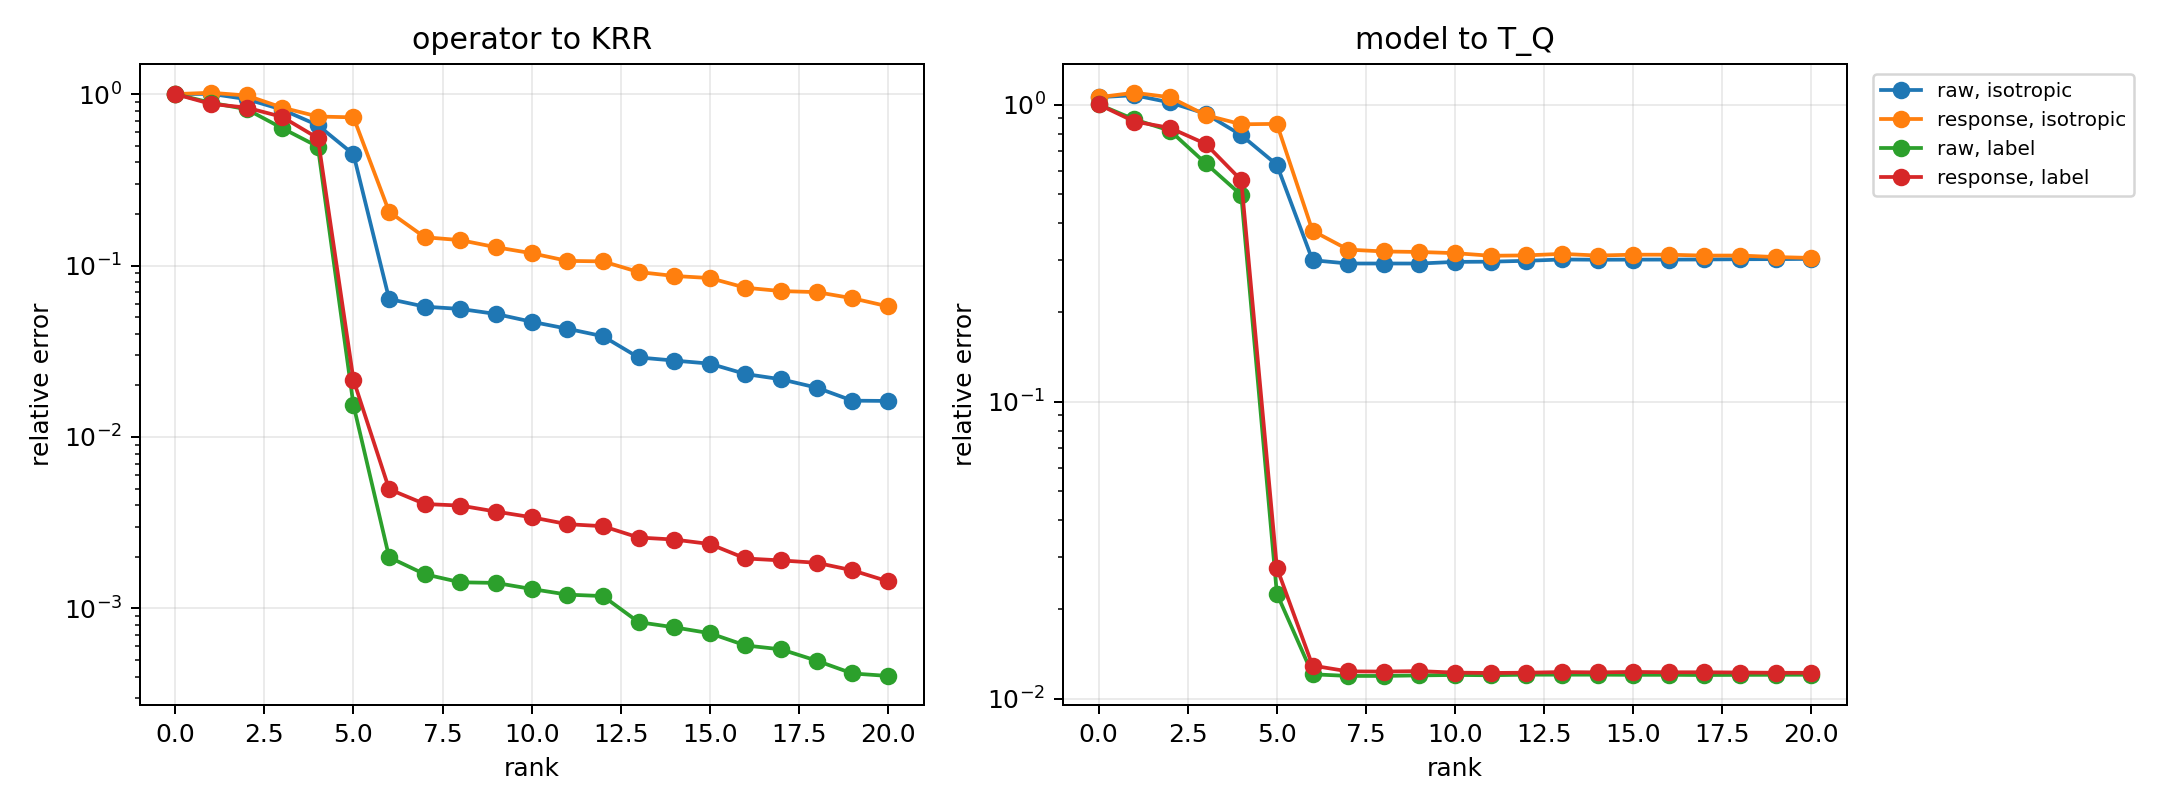
\includegraphics[width=\linewidth]{../experiments/exp1_operator_certificate/results/rank_curves.png}
\caption{Experiment 1 rank curves for raw and response-only final-state bases. The horizontal axis
is the retained basis rank \(r\).  At each \(r\), the experiment keeps the first \(r\) extracted
directions, forms \(T_Q=K_tQQ^\top\), and reevaluates the operator errors.  Left panel:
reduced-operator error \(E(T_Q,T)\), so this panel asks whether the retained final-state directions
are sufficient to reproduce ridge on the probe distribution.  Right panel:
transformer-to-reduced-operator response error \(E_\varepsilon(F,T_Q)\), so this panel asks whether
the transformer's local response follows that reduced operator.  The task-label curves drop sharply
once enough directions are retained, while the isotropic curves remain substantially larger.  This
shows both that the final residual stream exposes the task-relevant ridge directions and that these
directions do not explain arbitrary label perturbations equally well.}
\end{figure}

\FloatBarrier

\section{Experiment 2: Layerwise Span and Task-Visible Rank}

The second experiment asks how the needed directions appear across layers. More precisely, it asks
whether the trained transformer exposes a compact seed span of directly accepted residual-stream
directions, whether that span is on the task-visible scale predicted by the KRR spectrum, and whether
the reduced operator induced by that span approximates \(T\).

At layer \(\ell\), define the hidden finite-difference response
\[
Z_\ell(u)=
\frac{
H_\ell^{\mathrm{ctx}}(y+\varepsilon u)-H_\ell^{\mathrm{ctx}}(y-\varepsilon u)
}{2\varepsilon}.
\]
Stacking these responses over build probes gives \(M_\ell\), a matrix of context-position patterns
visible in layer \(\ell\) when labels are perturbed.

The construction processes layers sequentially. Before layer \(\ell\), directions already accepted
from earlier layers define a pre-existing \(A\)-orthonormal span \(Q_\ell^{\mathrm{pre}}\). The novel
part of the layer response is
\[
N_\ell
=
\left(I-Q_\ell^{\mathrm{pre}}(Q_\ell^{\mathrm{pre}})^\top A\right)M_\ell.
\]
An \(A\)-weighted SVD of \(N_\ell\) gives candidate directions. Visibility is not enough: a candidate
is accepted only if removing it from the context residual stream at that layer changes the
transformer's finite-difference response by a predeclared amount.

The accepted directions across layers define the seed layerwise activation span
\[
R_{\mathrm{seed}}=\spanop\{S_0,\ldots,S_L\},
\qquad
d_{\mathrm{seed}}=\dim R_{\mathrm{seed}}.
\]
Let \(Q_{\mathrm{seed}}\) be an \(A\)-orthonormal basis of this span and
\[
T_{Q_{\mathrm{seed}}}=K_tQ_{\mathrm{seed}}Q_{\mathrm{seed}}^\top.
\]
The diagnostic expectation is a post-training resource law with an alignment condition:
\[
d_{\mathrm{seed}}/r_{\mathrm{task}}\approx1
\quad\Longrightarrow\quad
E(T_{Q_{\mathrm{seed}}},T)\approx0,
\]
provided the selected span is aligned with the task-visible ridge directions. This is not an exact
rank identity. The seed span counts directions used by the trained transformer; \(r_{\mathrm{task}}\)
is the optimal ridge rank for task-distributed perturbations. Dimension by itself is not the
certificate; the reduced operator \(T_{Q_{\mathrm{seed}}}\) is the certificate.

The target-rank sweep supports this interpretation. Here \(r_T\) denotes the tail-based
task-visible rank at RMS tolerance \(\epsilon=0.01\), matching the definition above. For
\[
d_x\in\{3,5,8,10\},
\]
the seed span contains slightly more directions than the empirical task-visible rank and the
reduced-operator error is about \(10^{-3}\). This is the desired pattern: the model exposes a small
number of directly accepted residual-stream directions, those directions are on the same scale as
the ridge rank requirement, and restricting ridge to their span loses essentially none of the
task-local operator response. For \(d_x=15\), the seed span has enough dimension on average,
\[
d_{\mathrm{seed}}\approx15.8,
\qquad
r_{\mathrm{task}}\approx14.9,
\]
but the reduced-operator error rises to
\[
E(T_{Q_{\mathrm{seed}}},T)=0.08493.
\]
The failure is therefore not just a rank shortage. It says that the accepted seed directions have
enough dimension on average, but do not consistently span all task-visible ridge directions.

\begin{table}[htbp]
\centering
\caption{Experiment 2 complete target-rank sweep with causal seed-span selection, mean over 16
episodes per setting.}
\scriptsize
\setlength{\tabcolsep}{2.5pt}
\renewcommand{\arraystretch}{0.85}
\scalebox{0.84}{%
\begin{tabular}{lrrrrrr}
\toprule
Setting & \(d_{\mathrm{seed}}\) & \(r_T\) & \(d_{\mathrm{seed}}/r_T\) &
\(E(T_Q,T)\) & \(E(F,T_Q)\) & \(E(F,T)\)\\
\midrule
\(d_x=3\) & 4.6 & 3.0 & 1.542 & 0.00114 & 0.00641 & 0.00629\\
\(d_x=5\) & 6.0 & 5.0 & 1.200 & 0.00135 & 0.00926 & 0.00911\\
\(d_x=8\) & 9.0 & 8.0 & 1.125 & 0.00174 & 0.01317 & 0.01293\\
\(d_x=10\) & 11.0 & 10.0 & 1.100 & 0.00135 & 0.01309 & 0.01305\\
\(d_x=15\) & 15.8 & 14.9 & 1.063 & 0.08493 & 0.09598 & 0.01743\\
\(d_x=30\) & 47.0 & 16.0 & 2.938 & 0.00000 & 1.68673 & 1.68673\\
\bottomrule
\end{tabular}}
\renewcommand{\arraystretch}{1}
\end{table}

The \(d_x=30\) row is an exploratory stress case. Since \(n_{\mathrm{tgt}}=16\), the task-visible
rank is capped at \(r_T=16\), even though the input dimension is 30. In the seed-span rerun, causal
selection expands to the full context-position space, \(d_{\mathrm{seed}}=47\), so the reduced
operator equals exact KRR by construction:
\[
E(T_Q,T)=0.
\]
But the model itself is not behaviorally close to ridge:
\[
E(F,T)=1.68673.
\]
This is a useful stress-test warning. A large or even full seed span can make \(T_Q\) ridge-sufficient
without showing that the transformer uses that operator. The model-subspace alignment error
\[
E(F,T_Q)=1.68673
\]
exposes the failure.
Thus \(d_x=30\) reinforces the diagnostic separation: representation sufficiency is not behavioral
success, and dimension alone is not the mechanism claim.

\begin{table}[htbp]
\centering
\caption{Experiment 2 fixed-\(d_x=5\) depth/head sweep with causal seed-span selection, mean over
16 episodes. All checkpoints use width \(D=128\).}
\scriptsize
\setlength{\tabcolsep}{2.5pt}
\renewcommand{\arraystretch}{0.85}
\scalebox{0.84}{%
\begin{tabular}{lrrrrrrr}
\toprule
Checkpoint & \(L\) & \(H\) & \(d_{\mathrm{seed}}\) & \(r_T\) & \(E(T_Q,T)\) &
\(E(F,T_Q)\) & \(E(F,T)\)\\
\midrule
\(L=2\)  & 2  & 4 & 16.3 & 5.0 & 0.00095 & 0.18537 & 0.18535\\
\(L=4\)  & 4  & 4 & 6.2  & 5.0 & 0.00127 & 0.02534 & 0.02528\\
\(L=6\)  & 6  & 4 & 6.1  & 5.0 & 0.00137 & 0.01272 & 0.01255\\
\(L=8\)  & 8  & 4 & 6.0  & 5.0 & 0.00147 & 0.00962 & 0.00952\\
\(L=12\) & 12 & 4 & 6.1  & 5.0 & 0.00110 & 0.00953 & 0.00943\\
\(H=1\)  & 8  & 1 & 6.2  & 5.0 & 0.00085 & 0.01558 & 0.01559\\
\(H=2\)  & 8  & 2 & 6.1  & 5.0 & 0.00108 & 0.00908 & 0.00904\\
\(H=8\)  & 8  & 8 & 6.0  & 5.0 & 0.00164 & 0.00996 & 0.00982\\
\bottomrule
\end{tabular}}
\renewcommand{\arraystretch}{1}
\end{table}

The fixed-\(d_x=5\) depth and head sweeps add an important qualification. These checkpoints keep
the task dimension and width fixed while varying depth over \(L\in\{2,4,6,8,12\}\) and head count
over \(H\in\{1,2,4,8\}\). Causal seed selection gives \(E(T_Q,T)\approx10^{-3}\) for all reported
checkpoints, but behavior still varies: the shallow \(L=2\) model has a strong reduced-operator
certificate but
\(E(F,T)=0.185\), while the \(L=8\), \(H=2\), and \(L=12\) checkpoints have errors near \(10^{-2}\).
Thus the sweep is a control against conflating availability with use:
\[
E(T_Q,T)\ \text{small}
\]
does not imply
\[
E_\varepsilon(F,T)\ \text{small}.
\]
The activations may expose a ridge-sufficient subspace even when the trained transformer does not
use it accurately enough to behave like KRR.

\section{Dimension-40 Regime-Mismatch Stress Test}

The \(d_x=40\) checkpoint is useful because it separates two questions that are easy to conflate:
whether KRR-relevant directions are present in the residual stream, and whether the trained model
uses them as a full target-rich KRR operator. The checkpoint was trained in a target-poor regime:
\[
n_{\mathrm{tgt}}=8,
\qquad
\tau(\Sigma)=\sum_{i=1}^{40}\frac{\lambda_i}{\lambda_i+\sigma^2}\le16,
\]
with \(n_{\mathrm{ctx}}\) sampled as a multiple of the effective dimension. Thus each training episode
directly supervised only a small number of target queries. Across many episodes this is still a
Monte Carlo signal for the population prediction loss, but it does not force one forward pass to
expose a high-rank simultaneous target operator.

The diagnostic deliberately uses a richer geometry:
\[
n_{\mathrm{ctx}}=47,\qquad n_{\mathrm{tgt}}=40.
\]
In this setting the task-visible rank is
\[
r_T=32.4,
\]
well above the training target count. Hence the diagnostic is a stress test of whether a
target-poor-trained checkpoint generalizes to a much richer finite-episode operator.

\begin{table}[htbp]
\centering
\caption{\(d_x=40\) target-rich diagnostics. The first two rows come from the final-state
certificate run. The causal seed rows come from a separate 16-episode causal run; both arithmetic
means and medians are shown because two catastrophic episodes dominate the mean. Within a single
run, \(E(F,T)\) is independent of the chosen basis.}
\scriptsize
\setlength{\tabcolsep}{2.4pt}
\renewcommand{\arraystretch}{0.9}
\begin{tabular}{llrrrrrr}
\toprule
Run & Basis & Statistic & \(\dim Q\) & \(r_T\) & \(E(T_Q,T)\) & \(E(F,T_Q)\) & \(E(F,T)\)\\
\midrule
Final-state & raw & mean & 40.0 & -- & 0.01922 & 0.08512 & 0.08541\\
Final-state & response & mean & 40.0 & -- & 0.07400 & 0.11286 & 0.08541\\
Causal seed & seed & mean & 29.2 & 32.4 & 0.13741 & 98.74530 & 98.67662\\
Causal seed & seed & median & 28.0 & 35.0 & 0.17142 & 0.21569 & 0.12781\\
\bottomrule
\end{tabular}
\renewcommand{\arraystretch}{1}
\end{table}

The final-state certificate shows availability. At rank \(40\), the raw final-state basis induces a
reduced KRR operator close to exact KRR on task-label probes:
\[
E(T_{Q_{\mathrm{raw}}},T)=0.01922.
\]
The response-only final basis is weaker but still informative,
\[
E(T_{Q_{\mathrm{resp}}},T)=0.07400.
\]
These numbers say that the final residual stream contains many context-position directions from
which a KRR-structured operator can be built. The common value of \(E(F,T)\) across the two
final-state rows is expected, because \(E(F,T)\) does not depend on whether the comparison basis is
raw or response-only. These final-state rows do not say that the transformer uses those directions
causally, and they also use a broad rank cap \(40\), not the task-visible rank itself.

The causal target-rich diagnostic gives the harder reading, but the arithmetic mean must be read
carefully. It accepts
\[
d_{\mathrm{seed}}=29.2
\]
directions on average, while KRR requires
\[
r_T=32.4
\]
task-visible directions at the reported tolerance. The dimension ratio is therefore about \(0.90\).
The median episode is similar in scale, with \(d_{\mathrm{seed}}=28.0\) and \(r_T=35.0\). Moreover,
\[
E(T_{Q_{\mathrm{seed}}},T)=0.13741,
\]
with median \(0.17142\), so the accepted span is not merely a little short; it is also not perfectly
aligned with the task-visible KRR directions.

The model-response mean is much less representative. The causal run contains two catastrophic
pointwise failures: episodes 3 and 15 have model/KRR MSE ratios \(3304.6\) and \(35537.9\),
respectively. These two episodes drive
\[
E(F,T)=98.67662.
\]
The median is instead
\[
E(F,T)=0.12781,
\]
and after excluding episodes with \(E(F,T)>1\), the mean over the remaining 14 episodes is
\[
E(F,T)=0.12346.
\]
Thus the target-rich causal diagnostic shows lack of robustness rather than uniform failure on every
episode: most episodes are moderately KRR-like, but rare scale/spectrum cases cause catastrophic
breakdown.

The interpretation is not that target-poor training is theoretically incapable of learning KRR.
Resampled small target sets can train the population prediction rule in expectation. The point is
mechanistic and operational: training with \(n_{\mathrm{tgt}}=8\) did not give strong per-episode
pressure to build a reusable \(r_T\approx32\) label-response operator. When the diagnostic removes
the target cap, it asks for a richer simultaneous computation than the checkpoint was directly
trained to expose. The \(d_x=40\) result should therefore be read as a regime-mismatch stress test:
the model contains substantial KRR-sufficient final-state structure, but the causal seed span is
short or misaligned relative to the target-rich \(r_T\), and the model has rare catastrophic failures
in this richer regime.

This motivates the sequence-length prescription above. If the goal is to train and certify a true
task-visible KRR mechanism in a given regime, choose \(n_{\mathrm{ctx}}\) and \(n_{\mathrm{tgt}}\) so that
\[
\min\{n_{\mathrm{ctx}},n_{\mathrm{tgt}},r_*(n_{\mathrm{ctx}};\epsilon)\}
=r_*(n_{\mathrm{ctx}};\epsilon)
\]
during training as well as diagnosis. Target-rich diagnostics alone can reveal the missing operator;
target-rich training is the direct way to put pressure on the model to learn it.

\section{RBF Kernel Experiment: Prediction-Risk Rank and Availability}

The RBF experiment tests whether the same operator picture survives when the task-visible rank is no
longer tied to the input dimension. The checkpoint is trained on labels from an RBF Gaussian process
with lengthscale \(3.0\), signal variance \(1.0\), and noise variance \(\sigma^2=0.1\). On held-out RBF
tasks the model is close to KRR: at the end of training the prediction MSE is within about
\(1\)--\(3\%\) of exact KRR, and the model--KRR prediction discrepancy is around \(10^{-3}\).

For this nonlinear task, the strict rank used above,
\[
r_{1\%\mathrm{op}}
=
\min\left\{r:
\sqrt{\frac{\sum_{i>r}s_i^2}{\sum_i s_i^2+\eta_{\mathrm{num}}}}
\le 0.01
\right\},
\]
is a deliberately stringent operator-completion diagnostic. It asks for one-percent relative
operator recovery even when the omitted modes are below the task's prediction noise scale. For the
RBF task we therefore also compute the prediction-risk rank
\[
r_{5\%}
=
\min\left\{r:\sum_{i>r}s_i^2\le 0.05\,R_{\mathrm{KRR}}\right\},
\qquad
R_{\mathrm{KRR}}
=
\operatorname{tr}\!\left(K_{tt}-K_tA^{-1}K_t^\top\right).
\]
This is model-independent: it is computed from the KRR geometry before looking at activations. It
asks how many modes are needed so that discarding the rest would add at most five percent of the KRR
posterior prediction risk. Equivalently, it induces an episode-dependent operator tolerance
\[
\tau_{\mathrm{task}}
=
\sqrt{\frac{0.05\,R_{\mathrm{KRR}}}{\sum_i s_i^2+\eta_{\mathrm{num}}}}.
\]
In the RBF spectral scan this tolerance is much looser than \(0.01\): about \(0.064\) for
\(n_{\mathrm{ctx}}=47\) and about \(0.044\) for \(n_{\mathrm{ctx}}=128\). This is the missing
normalization. The strict rank counts low-energy tail modes; \(r_{5\%}\) counts modes that matter
relative to the irreducible KRR prediction risk.

\begin{table}[htbp]
\centering
\caption{RBF diagnostics. \(r_{5\%}\) is the prediction-risk rank; \(r_{1\%\mathrm{op}}\) is the old
strict relative-operator rank. The final-state column reports the raw final-basis reduced-operator
error at the nearest rank to \(r_{5\%}\). The causal seed columns use the layerwise causal extractor
and should be read as a stricter mechanistic test, not as the definition of task rank.}
\scriptsize
\setlength{\tabcolsep}{3pt}
\renewcommand{\arraystretch}{0.9}
\begin{tabular}{lrrrrrr}
\toprule
Regime & \(r_{5\%}\) & \(r_{1\%\mathrm{op}}\) & raw final \(E(T_Q,T)\) &
\(d_{\mathrm{seed}}\) & seed \(E(T_Q,T)\) & MSE/KRR\\
\midrule
\(n_{\mathrm{ctx}}=47,\ n_{\mathrm{tgt}}=64\)   & 17.1 & 27.7 & 0.12095 & 19.8 & 0.14352 & 1.013\\
\(n_{\mathrm{ctx}}=47,\ n_{\mathrm{tgt}}=128\)  & 18.3 & 30.6 & 0.11393 & 21.1 & 0.13612 & 1.024\\
\(n_{\mathrm{ctx}}=128,\ n_{\mathrm{tgt}}=128\) & 24.8 & 47.1 & 0.07313 & 22.9 & 0.17226 & 1.052\\
\(n_{\mathrm{ctx}}=128,\ n_{\mathrm{tgt}}=256\) & 28.6 & 51.2 & 0.06499 & 23.0 & 0.16480 & 1.007\\
\bottomrule
\end{tabular}
\renewcommand{\arraystretch}{1}
\end{table}

The table gives a clean reading. First, the RBF behavior itself is strong: the model's MSE is close
to KRR in all four evaluations. Second, the rank requirement is not the strict operator rank. Under
the prediction-risk definition, the relevant ranks are roughly \(17\)--\(29\), not \(28\)--\(51\).
Thus it is not paradoxical that a compact representation could support near-KRR prediction while
failing to recover every strict tail mode.

Third, the final residual stream contains substantial RBF-KRR structure. At the prediction-risk
rank, the raw final-state basis already reduces the KRR operator error to \(0.06\)--\(0.12\), and
the full rank curves continue down to exact operator recovery when the retained basis spans the
context-position space. This is an availability result: the information needed to build the RBF KRR
operator is present in the final context states to a significant degree. It is weaker than the linear
certificate, where the reduced-operator error is essentially numerical zero at the task rank, but it
is far from a failure.

The unresolved part is the causal seed extractor. Its dimension is close to \(r_{5\%}\) in the
\(n_{\mathrm{ctx}}=47\) runs and slightly short in the \(n_{\mathrm{ctx}}=128\) runs, but the induced
operator error remains around \(0.14\)--\(0.17\). This exceeds the implied prediction-risk operator
tolerance. Therefore the RBF causal span should not be claimed as a complete KRR mechanism. The
right interpretation is narrower and cleaner:
\[
\text{RBF behavior and final-state availability succeed,}
\]
while
\[
\text{causal seed extraction remains only partially aligned with the KRR operator.}
\]
This distinction is useful. It says the RBF checkpoint has learned near-KRR prediction and exposes
much of the relevant operator structure, but our current layerwise causal basis construction is not
yet a fully satisfactory mechanistic certificate for the nonlinear task.

\section{Experiment 4: Causal Direction Removal}

The fourth experiment asks whether the task-important directions inside \(Q\) are actually used by
the transformer. This is necessary because decodability and sufficiency do not by themselves prove
causal use.

Start with a raw final basis \(Q=[q_1,\ldots,q_r]\). For each direction, form \(Q_{-j}\) by removing
that column. The point of the leverage score is to rank directions by their importance to the
KRR-constrained reduced operator, not by activation magnitude. A direction should count as
task-important if deleting it changes \(T_Q\)'s response on task-label probes. Define
\[
\Lambda_j^{\mathrm{red}}(U)
:=
\left(
\frac{
\sum_{u\in U}\|(T_Q-T_{Q_{-j}})u\|_2^2
}{
\sum_{u\in U}\|Tu\|_2^2+\eta_{\mathrm{num}}
}
\right)^{1/2}.
\]
A direction has high task leverage if this score is large on task-label probes. This ranking is what
connects the causal intervention to the operator certificate: the surgery removes directions that
\(T_Q\) itself says are important for task-distributed ridge responses.

The intervention removes selected directions from the context-token residual stream:
\[
H_s^{\mathrm{ctx}}
\longmapsto
H_s^{\mathrm{ctx}}
-
\sum_{j\in J}q_jq_j^\top A H_s^{\mathrm{ctx}},
\]
then rolls the remaining layers forward. Matched controls remove low-task-leverage directions from
the same basis, high-isotropic-but-low-task directions, high-activation-variance-but-low-task
directions, and random subsets.

Before surgery, the checkpoint is in the task-local certificate regime:
\[
E_{\mathrm{task}}(F,T)=0.00926,
\qquad
E_{\mathrm{task}}(F,T_Q)=0.00920,
\qquad
E_{\mathrm{task}}(T_Q,T)=0.00086.
\]
The same episodes retain the off-distribution drift seen in Experiment 1:
\[
E_{\mathrm{iso}}(F,T)=0.266,
\qquad
E_{\mathrm{iso}}(T_Q,T)=0.0378.
\]
At residual state \(s=1\), removing a single high-task-leverage direction causes prediction drift
\(4.68\), KRR-error inflation \(649\times\), and task-response damage \(41.59\). Removing a
single low-task-leverage direction from the same basis is nearly inert: prediction drift
\(9.8\cdot10^{-4}\), KRR-error inflation \(1.03\times\), and task-response damage \(0.0024\).
The layer sweep localizes the effect: high-task surgery is most damaging at early residual states,
before later attention has routed the relevant context information into target tokens, and
context-only surgery after the final layer is a no-op. At \(s=1\), aggregate task leverage and task
response damage are strongly related across matched non-random controls (log--log Pearson 0.91,
Spearman 0.87).

The complement ablation sharpens the mediation claim. At the same residual state \(s=1\), keeping
only the \(A\)-projection of context residual states onto \(Q\),
\[
H_s^{\mathrm{ctx}}\mapsto QQ^\top A H_s^{\mathrm{ctx}},
\]
nearly preserves the task-local response over 8 episodes:
\[
E_{\mathrm{task}}(F,T)=0.01866,
\qquad
\text{response damage}=0.01659.
\]
Removing \(Q\) instead,
\[
H_s^{\mathrm{ctx}}\mapsto H_s^{\mathrm{ctx}}-QQ^\top A H_s^{\mathrm{ctx}},
\]
destroys the response:
\[
E_{\mathrm{task}}(F,T)=145.43,
\qquad
\text{response damage}=145.43.
\]
So the complement of \(Q\) is largely dispensable for the task-local KRR response in this
intervention family, while \(Q\) itself is necessary.

\begin{figure}[htbp]
\centering
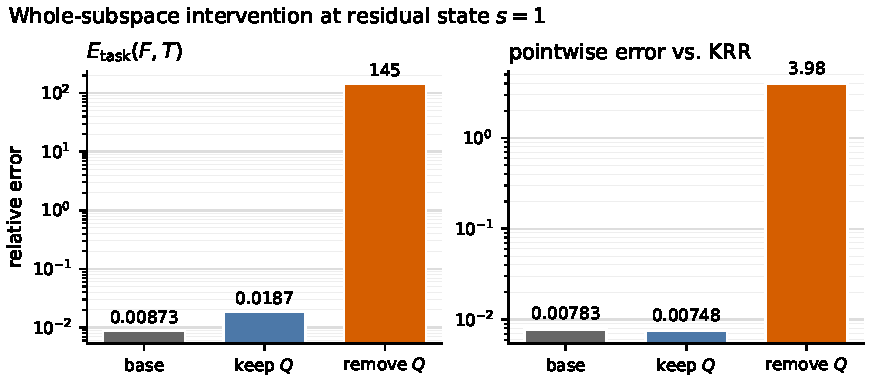
\includegraphics[width=0.82\linewidth]{../experiments/exp3_causal_surgery/results_complement_ablation/complement_ablation_bars.pdf}
\caption{Experiment 4: whole-subspace complement ablation at residual state \(s=1\). Left panel:
task finite-difference response error \(E_{\mathrm{task}}(F,T)\). Right panel: relative KRR
prediction error \(\|F_{\mathrm{surg}}(y)-Ty\|_2/\|Ty\|_2\). Keeping only the \(Q\)-projection
nearly preserves both quantities; removing \(Q\) destroys both.}
\end{figure}

\begin{figure}[htbp]
\centering
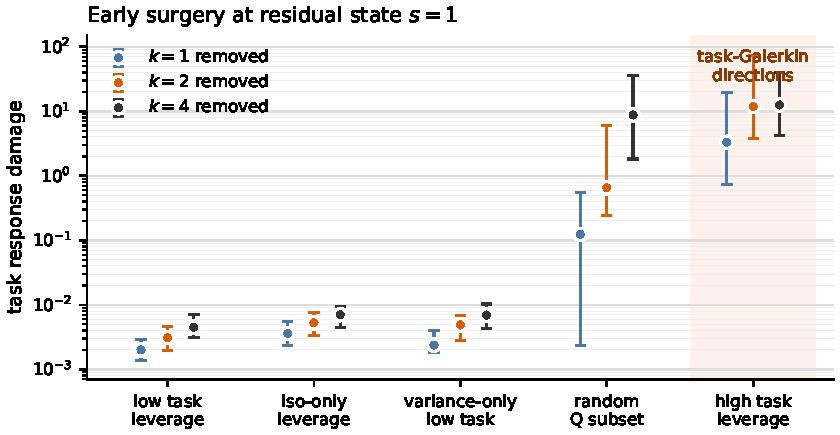
\includegraphics[width=0.78\linewidth]{../experiments/exp3_causal_surgery/results/experiment_3_key_surgery.pdf}
\caption{Experiment 4: causal effect of task-important activation directions. The plotted metric is
task finite-difference response damage
\(\bigl(\sum_j\|D_\varepsilon F_{\mathrm{surg}}(y)[u_j]-D_\varepsilon F_{\mathrm{base}}(y)[u_j]\|^2/
(\sum_j\|Tu_j\|^2+\eta_{\mathrm{num}})\bigr)^{1/2}\), for task probes \(u_j\sim\mathcal{N}(0,A)\).
High task-leverage directions produce orders-of-magnitude larger damage than low-task-leverage
directions from the same activation basis.}
\end{figure}

\begin{figure}[htbp]
\centering
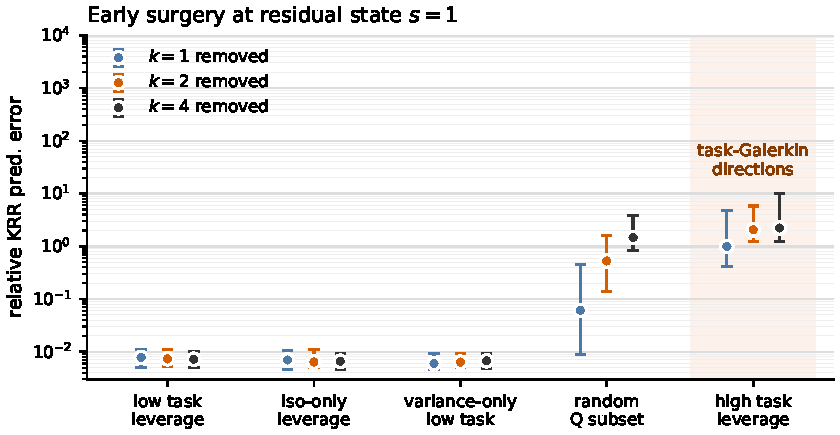
\includegraphics[width=0.78\linewidth]{../experiments/exp3_causal_surgery/results/experiment_3_key_surgery_point_error.pdf}
\caption{Experiment 4: the same surgery plot, but measuring relative KRR prediction error
\(\|F_{\mathrm{surg}}(y)-Ty\|_2/\|Ty\|_2\) instead of finite-difference response damage. High
task-leverage removals also destroy the model's prediction, while low-task-leverage removals are
nearly inert.}
\end{figure}

\FloatBarrier

This supports the causal-use claim in an operational sense. The directions that the reduced KRR
operator identifies as task-important are not merely decodable; removing them selectively damages
the transformer's task-local response, while matched controls do not.

\section{What Is Justified}

The experiments justify a bounded mechanistic claim:

\begin{quote}
For the tested checkpoint, geometries, perturbation scale, and task-label probe distribution, the
transformer's local label response is well approximated by a reduced KRR operator induced by a
compact context-side activation subspace. In successful settings the accepted seed span is on the
scale predicted by the task-visible KRR spectrum and its induced reduced operator is close to exact
KRR; its high-task-leverage directions are causally important for the transformer's response.
\end{quote}

They do not justify stronger claims. They do not show that the transformer globally equals ridge
regression. They do not show that derivative matching at one sampled label vector implies equality
on a neighborhood. They do not show that the transformer literally executes the explicit algorithm
\[
y\mapsto QQ^\top y\mapsto K_tQQ^\top y
\]
as its internal program. They also do not show that architecture alone guarantees the behavior.
The task-visible rank calculation supplies a requirement for context-side subspaces; it is not an
SGD theorem.

The clean final formulation is:

\begin{quote}
The trained transformer locally realizes the ridge-regression label-response operator on
task-distributed directions. In the tested regime, this behavior is explained by a compact
context-side activation subspace whose induced reduced ridge operator approximates exact KRR,
whose dimension is on the task-visible scale in successful settings, and whose high-leverage
directions are causally important for the transformer's response.
\end{quote}

\section{Logical Chain}

The argument can be read as a sequence of commitments, each narrower than the previous one:

\begin{enumerate}[label=\arabic*.]
\item Freeze the episode geometry \(G=(X_{\mathrm{ctx}},X_{\mathrm{tgt}})\).
\item Under fixed \(G\), ridge regression becomes \(T=K_tA^{-1}\).
\item Treat the transformer as a label map \(F:\R^{n_{\mathrm{ctx}}}\to\R^{n_{\mathrm{tgt}}}\).
\item Estimate the local response \(D_\varepsilon F(y)[u]\).
\item Test behavior by checking \(E_\varepsilon(F,T)\) on task-label probes.
\item Compute the task-visible rank from \(C_G=K_tA^{-1/2}\).
\item Extract activation-derived context-side bases \(Q\).
\item Construct the KRR-constrained reduced operator \(T_Q=K_tQQ^\top\).
\item Test subspace sufficiency with \(E(T_Q,T)\).
\item Test model-subspace alignment with \(E_\varepsilon(F,T_Q)\).
\item Compare seed layerwise span dimension \(d_{\mathrm{seed}}\) to \(r_{\mathrm{task}}\).
\item Remove high-leverage \(Q\)-directions and check whether task-local response is damaged.
\end{enumerate}

This is the full mechanism story: behavioral similarity, a KRR-structured activation certificate,
rank-scale agreement with the task-visible spectrum, and causal specificity of the high-leverage
directions.

\end{document}
